\section{Results}

Each of the classifiers described in \cref{models_section} was trained in a random subset of \num{50000} news samples for our dataset for 30 epochs.

The 30 epochs were more than enough, since we get the value from the epoch with the best validation score as described in \cref{early_stopping}.

\subsection{Seq2Seq and Transformer models}
Both the Seq2Seq and Transformer models seem to train slowly due to the large amount of data provided.

While we were not able to train many epochs due to technical reasons, this didn't seem to be necessary as both models have a minimal loss at epochs 11 and 14, respectively.

\begin{figure}[h]
	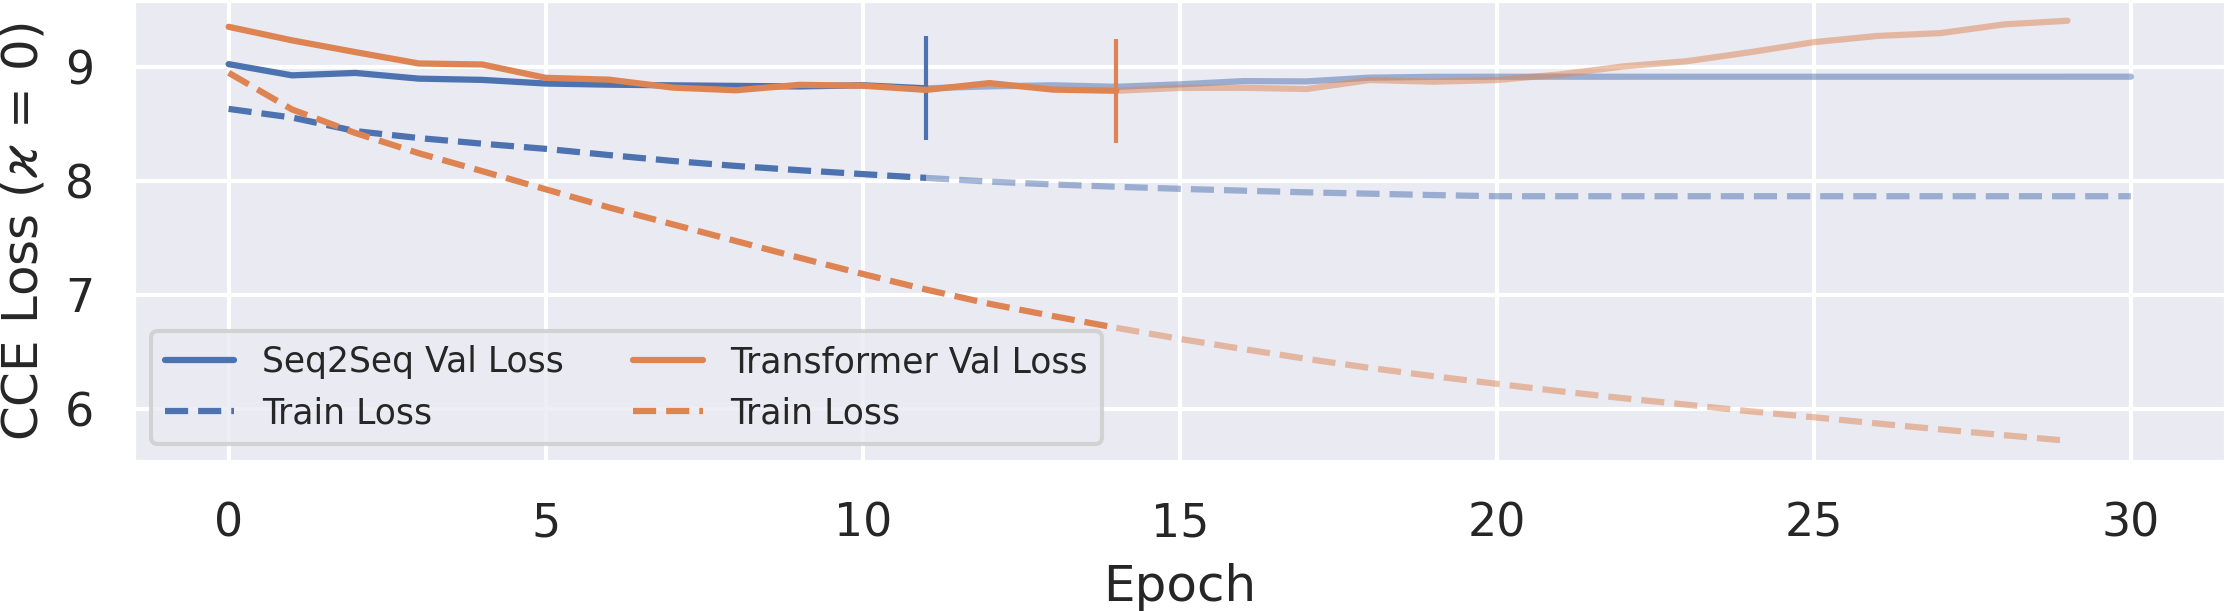
\includegraphics[width = \textwidth]{baseline_losses.png}
	\caption{Training and validation losses of both initial models. Due to early stopping, only the non-transparent part is considered.}
\end{figure}

While the categorical cross-entropy loss of these models seems similar, their ROUGE scores tell another story.
\Cref{baseline_rouges} contains the ROUGE-1 and ROUGE-2 scores of both models, where the transformer produces a considerably better score.

\begin{figure}[h]
	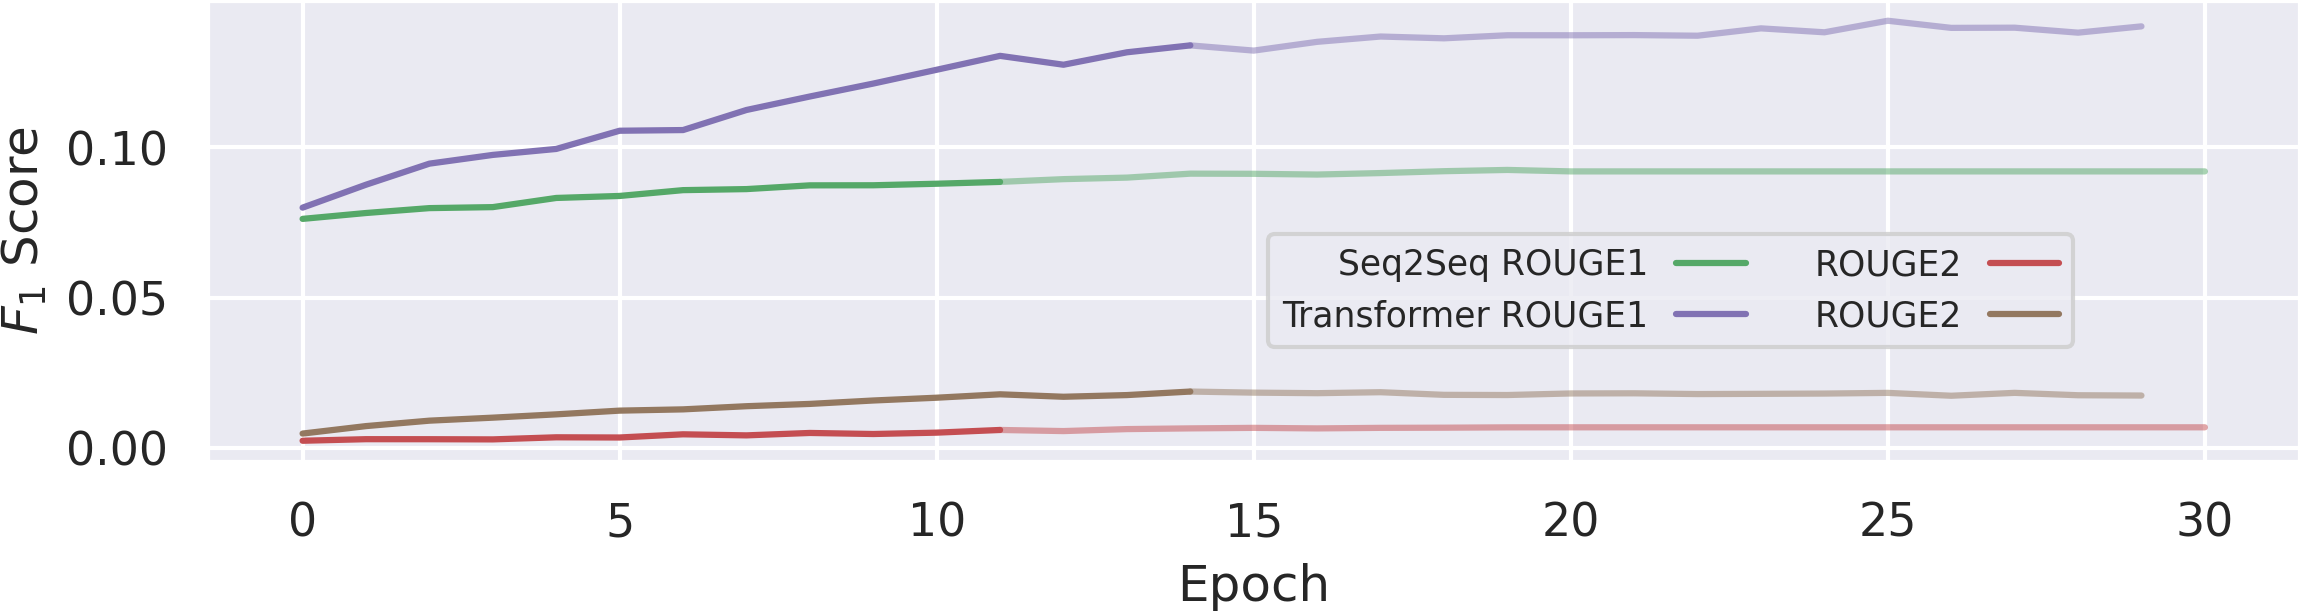
\includegraphics[width = \textwidth]{baseline_rouges.png}
	\caption{ROUGE scores of the Seq2Seq and Transformer models. The attention mechanism allows the transformer model to create more coherent result with higher ROUGE scores.}
	\label{baseline_rouges}
\end{figure}

Are these relatively good ROUGE scores good for having reasonable results?
The answer is a resounding \textbf{NO}.

\Cref{seq2seq_example,transformer_example} in \appendixA show some examples of the outputs from this model.
The results are nonsensical, and there is nothing that could even suggest where to start.

\subsection{BERTFormer}

With its pre-trained encoder, the BERTFormer model produced a better result than the regular Transformer model in both ROUGE scores.
However, it also gets to the best validation loss early, at epoch 12.

\begin{figure}[h]
	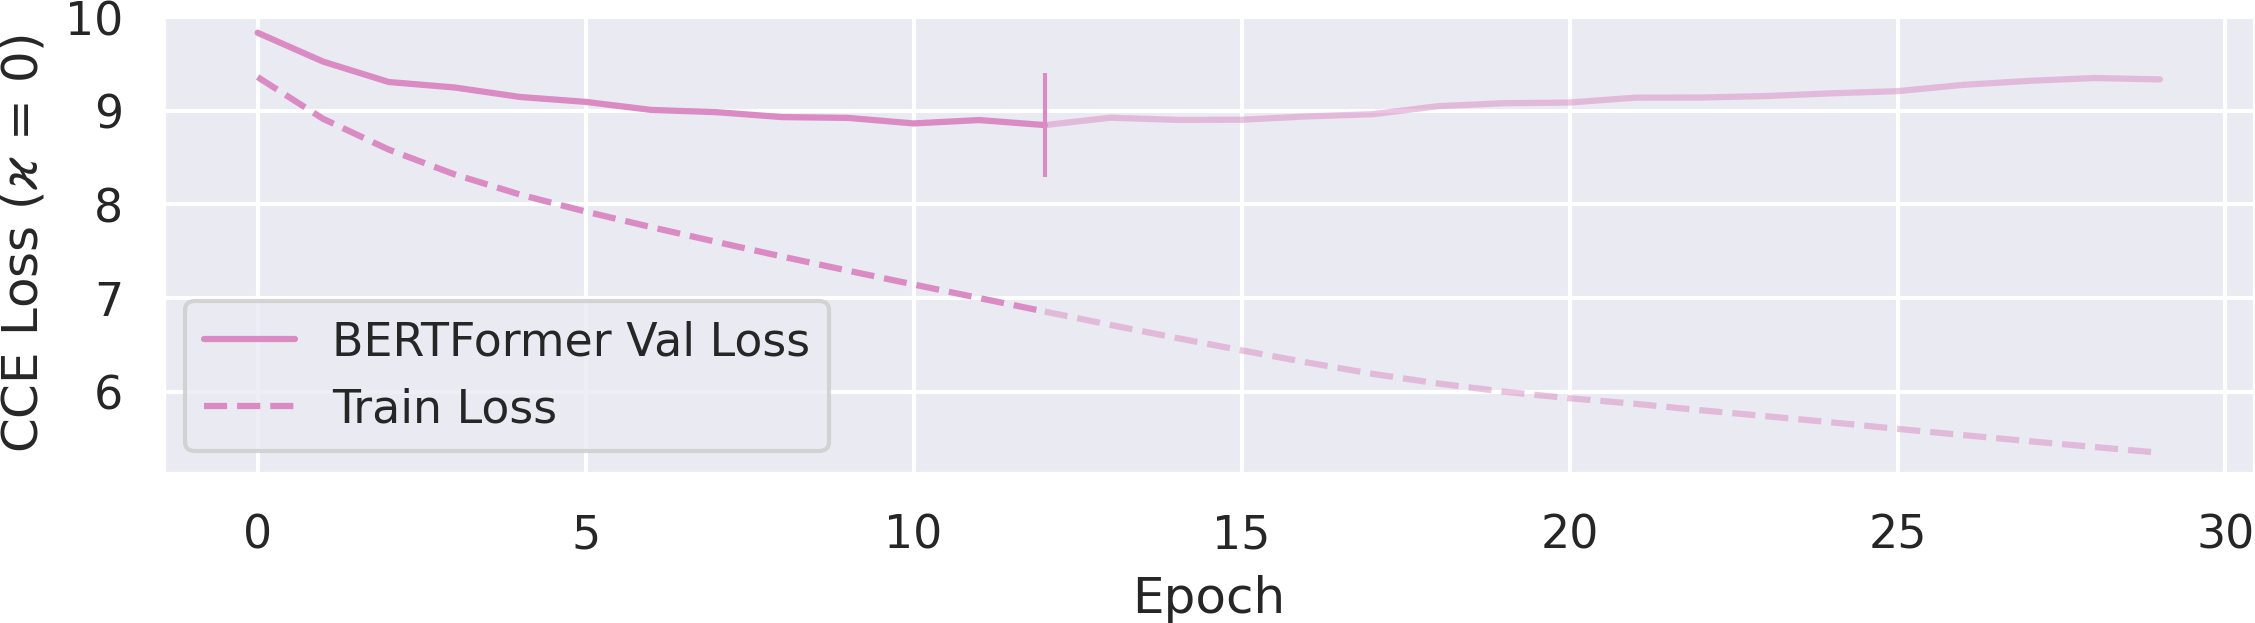
\includegraphics[width=\textwidth]{bertformer_loss.png}
	\caption{Training and validation loss of the BERTFormer transformer. It's notable that there is little change in the validation loss between epochs; this is likely an unfortunate artifact of the embeddings and the decoder of the classifier not learning much and categorical cross-entropy not being a good loss to minimise for this problem.}
\end{figure}

Despite this, it has significantly better ROUGE scores than the previous two classifiers, as can be seen in \cref{comparison_table}.

\begin{figure}[h]
	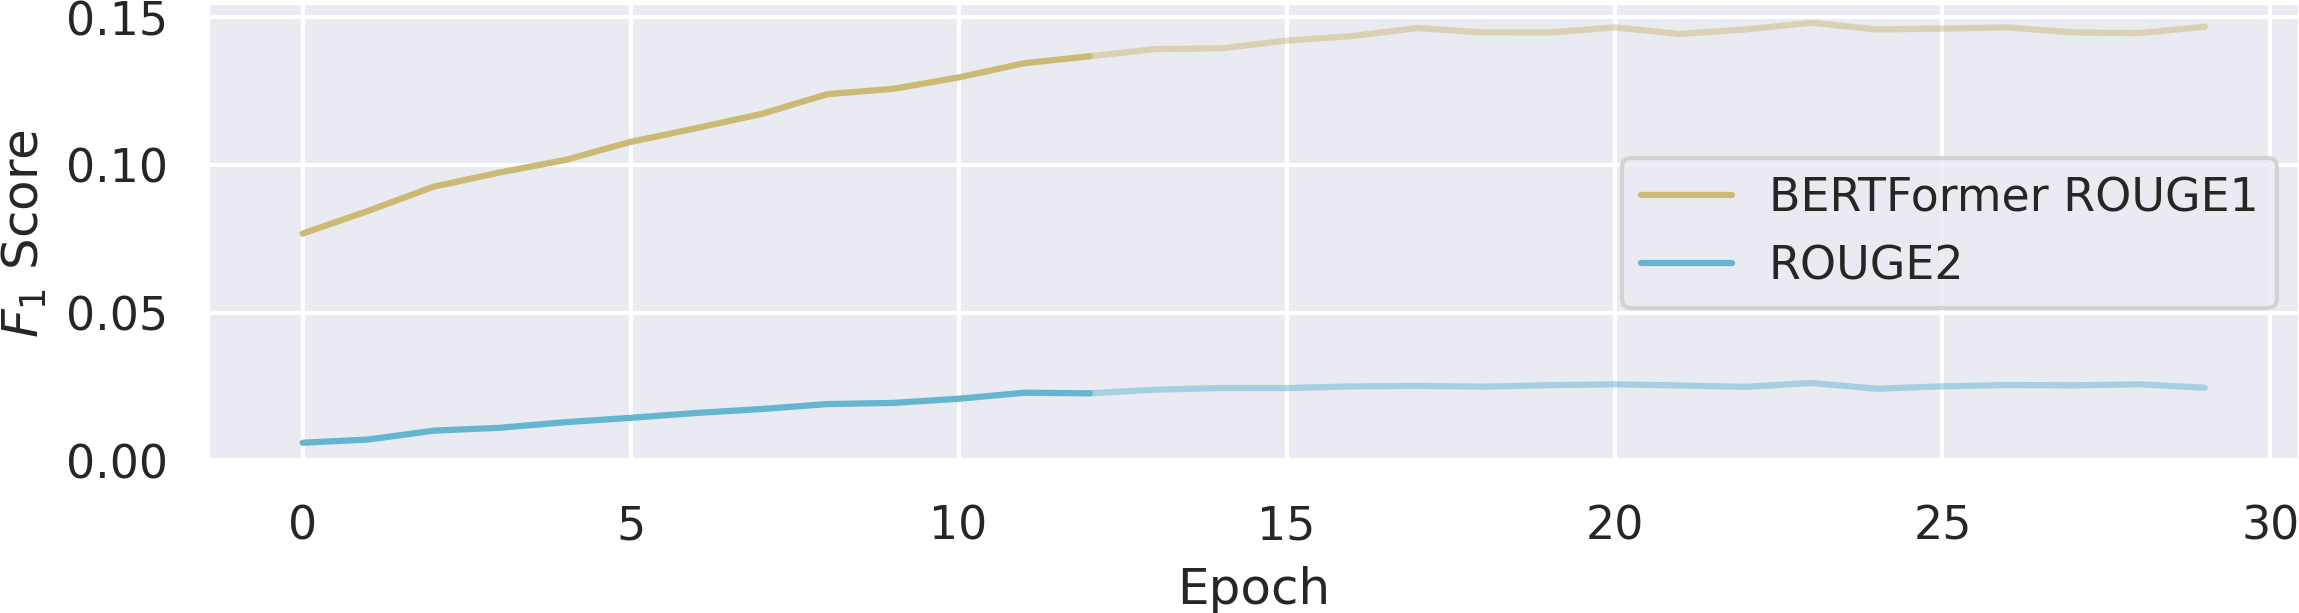
\includegraphics[width=\textwidth]{bertformer_rouge.png}
	\caption{ROUGE-1 and ROUGE-2 scores of the BERTFormer transformer, as it trains. The Rouge-1 score grows rapidly after the CCE loss stops growing and the training stops early; this is another proof that this loss might not be the best for this problem.}
\end{figure}

% \newpage{}
We can compare Cosine Similarity scores in \cref{cs_scores} with the transformer classifier to confirm that, while it's significantly better due to the BERT pre-trained embedding, it does not grow much as the model trains.

Why do the ROUGE scores improve as the model trains while the cosine similarity score doesn't? It's possible that the words predicted are ``close enough'' to the correct ones despite being wrong, althrough this seems to contradict the results of \appendixA{}. It's also possible that the embedding layer is not being trained sufficiently, which causes a collapse in the spatial dimensions and generally high CS scores for bad results.

\begin{figure}[h]
	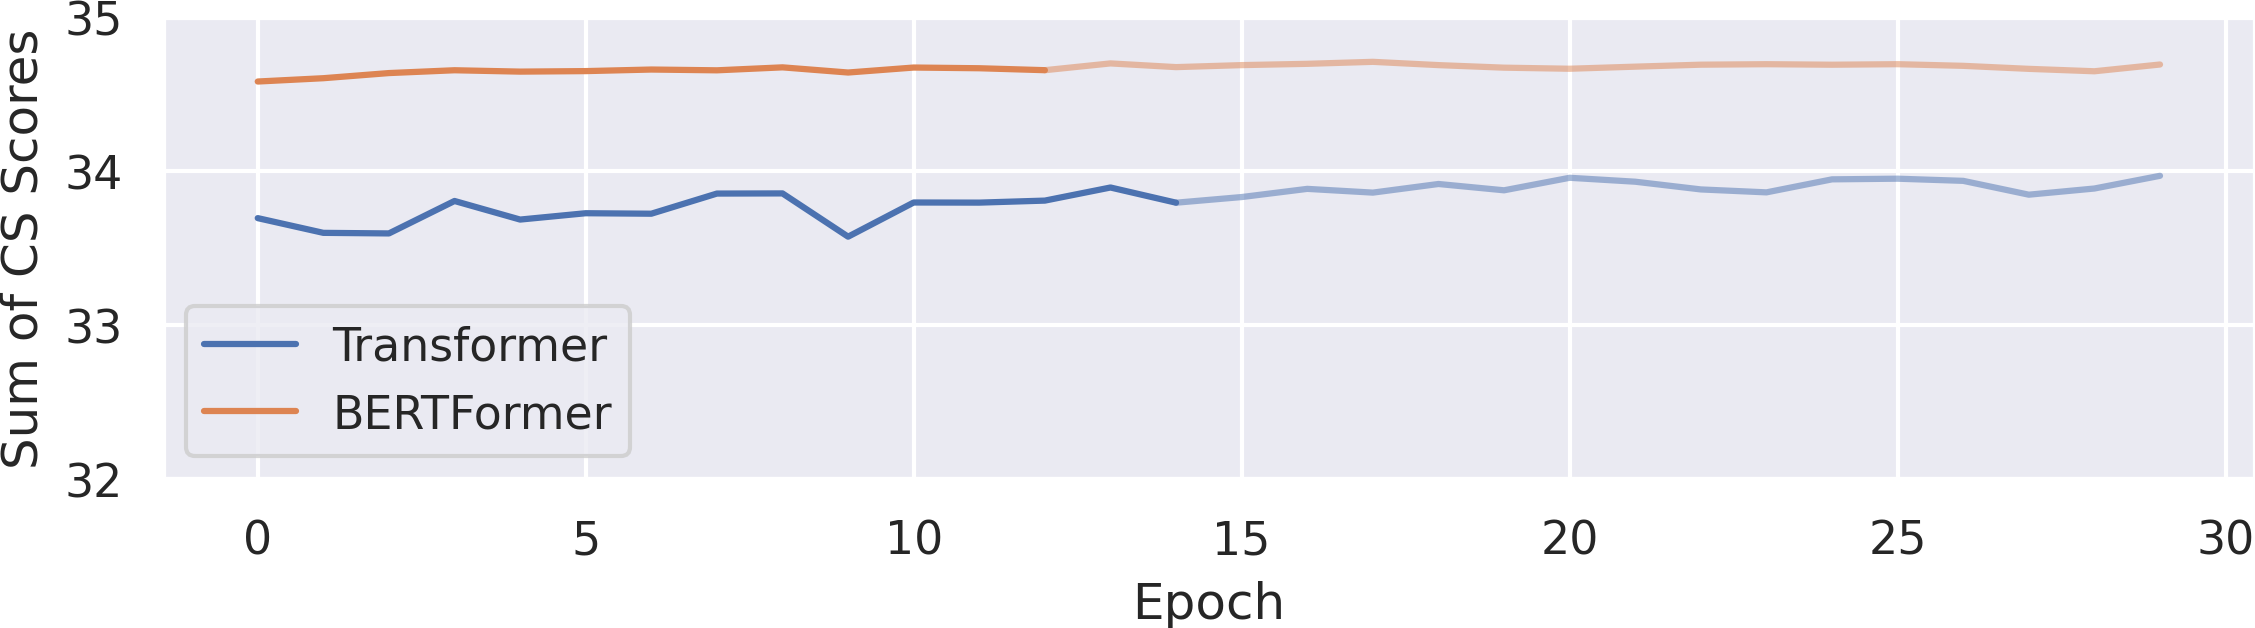
\includegraphics[width=\textwidth]{cs_scores.png}
	\caption{Cosine similarity scores of Transformer and BERTFormer models. The pretrained BERT encoder provides a significant advantage in guessing a result that's ``close'' to the target one; however, this advantage does not seem to grow as it trains unlike the ROUGE scores.}
	\label{cs_scores}
\end{figure}

\subsection{Final Results}
The final results contain a small but significant advantage in the BERTFormer model for all metrics.

\begin{table}[h]
	\centering
	\begin{tabular}{l | c c c c}
		\toprule
			Model & CCE & ROUGE-1 & ROUGE-2 & CS Score Sum \\
		\midrule
			Seq2Seq & 8.809 & 0.088 & 0.006 & N/A\footnotemark{} \\
			Transformer & 8.787 & 0.134 & 0.019 & 33.79 \\
			BERTFormer & 8.846 & 0.137 & 0.023 & 34.68 \\
		\bottomrule
	\end{tabular}
	\caption{Comparison of final scores between models. See \appendixA{} for text examples.}
	\label{comparison_table}
\end{table}

Sadly, this model keeps giving nonsensical and unworkable results, as seen in \cref{bertformer_example} in \appendixA{}.
Some reflections to the causes of this result and how to possibly fix them appear in \cref{reflections_section}.

\footnotetext{Our implementation of cosine similarity scores requires the output of the decoder as the representation of the entire sequence. It's not easy to think of a reasonable implementation of this in our Seq2Seq model, so this score is not calculated for this model.}
